
\documentclass[a4paper, 10pt]{article}

\usepackage{graphicx}
\usepackage[polish]{babel}
\usepackage[utf8]{inputenc}
\usepackage[OT4]{fontenc}
\usepackage{geometry}
\usepackage{ulem}
\usepackage{algorithm}
\usepackage{algorithmic}
\usepackage[section]{placeins}
\usepackage{amsmath}

\RequirePackage{url}


\setlength{\parindent}{0cm}
\setlength{\parskip}{3mm plus1mm minus1mm}

\geometry{verbose,a4paper,tmargin=2.3cm,bmargin=2.3cm,lmargin=2.4cm,rmargin=2.4cm}
\usepackage{graphicx} % wstawianie obrazkow


%%%%%%%%%%%%%%%%%%%%%%Do Pseudokodu%%%%%%%%%%%%%%%%%%%%%%%%%%%

\renewcommand{\algorithmicrequire}{\textbf{Dane wejściowe:}}
\renewcommand{\algorithmicensure}{\textbf{Inicjalizacja:}}
\renewcommand{\algorithmicend}{\textbf{end}}
\renewcommand{\algorithmicif}{\textbf{if}}
\renewcommand{\algorithmicthen}{\textbf{then}}
\renewcommand{\algorithmicelse}{\textbf{else}}
\renewcommand{\algorithmicelsif}{\algorithmicelse\ \algorithmicif}
\renewcommand{\algorithmicendif}{\algorithmicend\ \algorithmicif}
\renewcommand{\algorithmicfor}{\textbf{for}}
\renewcommand{\algorithmicforall}{\textbf{for all}}
\renewcommand{\algorithmicdo}{\textbf{do}}
\renewcommand{\algorithmicendfor}{\algorithmicend\ \algorithmicfor}
\renewcommand{\algorithmicwhile}{\textbf{while}}
\renewcommand{\algorithmicendwhile}{\algorithmicend\ \algorithmicwhile}
\renewcommand{\algorithmicloop}{\textbf{loop}}
\renewcommand{\algorithmicendloop}{\algorithmicend\ \algorithmicloop}
\renewcommand{\algorithmicrepeat}{\textbf{repeat}}
\renewcommand{\algorithmicuntil}{\textbf{until}}
\renewcommand{\algorithmicprint}{\textbf{print}}
\renewcommand{\algorithmicreturn}{\textbf{Wyjście:}}
\renewcommand{\algorithmictrue}{\textbf{true}}
\renewcommand{\algorithmicfalse}{\textbf{false}}

    
\floatname{algorithm}{}
\renewcommand\thealgorithm{}



%%%%%%%%%%%%%%%%%%%%%%%%%%%%%%%%%%%%%%%%%%%%%%%%



%%%%%%%%%%%%%%%%%%%%%%%%%%%%%%%%%%%%%%%%%%%%%%%%


\title{{\bf {Grafy i sieci}} \\ {\large Sprawozdanie końcowe}}
\date{\today}
\author{Filip Nabrdalik}

%%%%%%%%%%%%%%%%%%%%%%%%%%%%%%%%%%%%%%%%%%%%%%%%
\begin{document}
\bibliographystyle{plain}


%%%%%%%

\maketitle 


%%%%%%%%%%%%%%%%%%%%%%%%%%%%%


\newcommand{\ang}[1]{(ang.  #1\/)}
\newcommand{\e}[1]{{\em #1}\/}

\renewcommand*{\figurename}{Wykres}



\section{Treść zadania}

{\bf{Zadanie}}

Porównanie algorytmów znajdowania minimalnego drzewa rozpinającego.

{\it Wybrać, zaimplementować i przebadać co najmniej dwa algorytmy znajdowania minimalnego drzewa rozpinającego w grafie nieskierowanym. }

 

\section{Uwagi wstępne}

Niestety w wyniku zniejszenia zespołu projektowego o połowę nie udało sie zrealizować i ocenić algorytmu Borůvki. 
Na ostatnim etapie projektu zmieniły się również decyzje projektowe dotyczące użytych struktur danych, więc 
dokumentacja ta stanowi zarazem ostateczne sprawozdanie oraz doprecyzowanie poprzedniego dokumentu projektowego.



\section{Struktury danych i złożoność obliczeniowa}

Podczas prac projektowych okazało się, że użycie tylko jednej reprezentacji grafu jest niewystarczające. Do realizacji algorytmów należało użyć
list sąsiedztwa wierchołków oraz reprezentacji krawędziowej grafu. Dodatkowo należało też zmienić struktury danych używane do realizacji algorytmu Kruskala
i Prima.


{\bf{Algorytm Prima}}
 
 Do realizacji algorytmu zostały użyte listy sąsiedztwa wierzchołków.
 W celu zmniejszenia złożoności obliczeniowej struktura zbioru wierchołków Set $O(V^2)$ została zastąpiona
 przez kopiec binarny i przeszukiwanie wszerz BFS \ang{Breadth-first search}CITE. Przeszukiwanie wszerz jest wykorzystywane do
 poruszania sie po wierzchołkach $O(V+E)$, a kopiec binarny przechowuje wierchołki, które nie znajdują się w MST. Kopiec binarny używany 
 jest tu jako kolejka priorytetowa, aby szybko uzyskać krawędź o najmniejszej wadze $O(LogV)$. Złożoność obliczeniowa algorytmu powinna wynosić
 $O(ElogV)$.
 


{\bf{Algorytm Kruskala}}

Do realizacji algorytmu została wykorzystana reprezentacja krawędziowa grafu oraz struktura zbiorów rozłącznych. 
Dodatkową techniką używana w algorytmie jest scalenie poprzez rangę \ang{union by rank}, która pozwala na dołączenie mniejszego drzewa 
do korzenia większego $O(logV)$ CITE oraz kompresja ścieżki \ang{path compression} polegająca na "spłaszczeniu" drzewa podczas przeszukiwania  poprzez dołączanie 
odwiedzonych wierzchołków bezpośrednio do korzenia.łożoność obliczeniowa algorytmu powinna wynosić $O(ElogE)$.


%struktura zbiorow rozlacznych
%path compression

\section{Opis programu}

{\bf{Format danych wejściowych}}

Grafy sa reprezentowane w postaci krawędziowej w pliku tekstowym, której
każdy wiersz stanowi odrębną krawędź. Pierwsza i druga kolumna to numery wierzchołkow pomiędzy którymi istnieje krawędź.
Kolumna trzecia zawiera wagę wierchołka w postaci całkowitoliczbowej.

{\bf{Program mst}}

W celu uruchomienia algorytmów należy użyć polecenia: \\
{\it mst nazwa\_pliku\_grafu.txt k lub p}, \\
gdzie p oznacza użycie algorytmu Prima, a k Kruskala.





\section{Testy}
\subsection{Testy poprawności}
\subsection{Testy wydajnościowe}

\subsection{Zużycie pamięci}

\section{Wyniki}

\subsection{Czas wykonania}

\begin{center}
    \begin{tabular}{| l | l | c | c |}
    \hline
    V & p & Prim [ms] & Kruskal [ms] \\ \hline
	500 & 0.1 & 2 & 14  \\ 
	500 & 0.3 & 7& 23  \\ 
	500 & 0.5 & 14& 41  \\ 
	500 & 0.7 & 20& 53  \\ 
	500 & 0.9 & 30& 70  \\ \hline
	1000 & 0.1 & 17& 49  \\ 
	1000 & 0.3 & 49& 132  \\ 
	1000 & 0.5 & 62& 155 \\ 
	1000 & 0.7 & 75& 159 \\ 
	1000 & 0.9 & 120& 220  \\ \hline
	2000 & 0.1 & 39& 94  \\ 
	2000 & 0.3 & 116& 239  \\ 
	2000 & 0.5 & 183& 380  \\ 
	2000 & 0.7 & 259& 540  \\ 
	2000 & 0.9 & 329& 730  \\ \hline
	3000 & 0.1 & 82& 161\\ 
	3000 & 0.3 & 256& 521  \\ 
	3000 & 0.5 & 439& 895  \\ 
	3000 & 0.7 & 611& 2615  \\ \hline
    \end{tabular}
\end{center}



\begin{figure}[ht!]
\centering
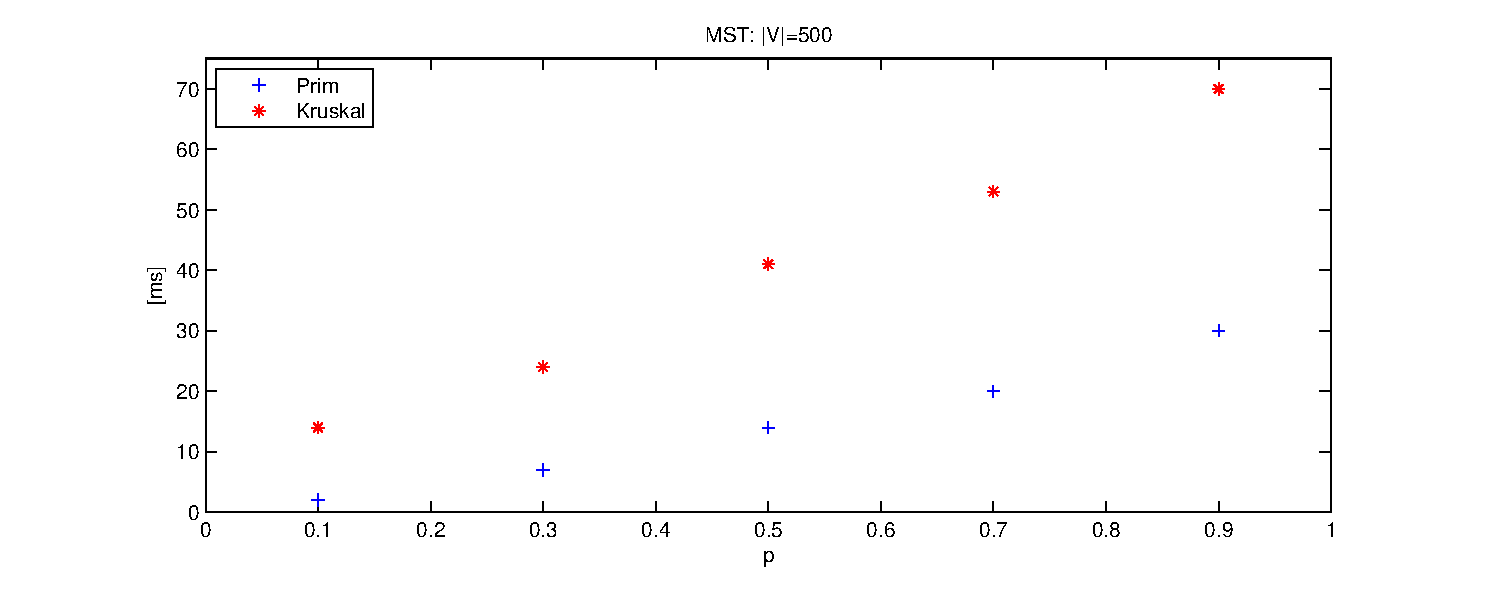
\includegraphics[width=165mm]{wykresy/v500.eps}
\caption{\it{Czas wykonania algorytmów dla grafu zawierającego 500 wierzchołków w zależności od prawdopodobieństwa wystąpienia krawędzi}}
\label{overflow}
\end{figure}

\begin{figure}[ht!]
\centering
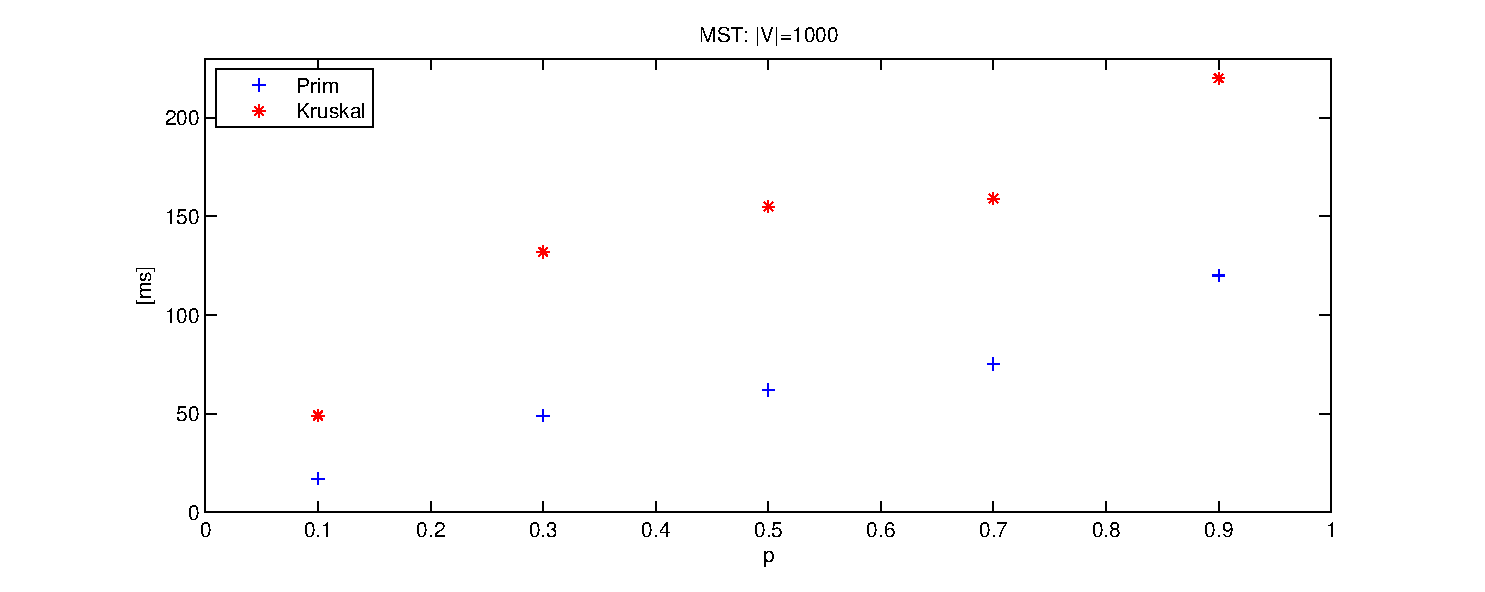
\includegraphics[width=165mm]{wykresy/v1000.eps}
\caption{\it{Czas wykonania algorytmów dla grafu zawierającego 1000 wierzchołków w zależności od prawdopodobieństwa wystąpienia krawędzi}}
\label{overflow}
\end{figure}

\begin{figure}[ht!]
\centering
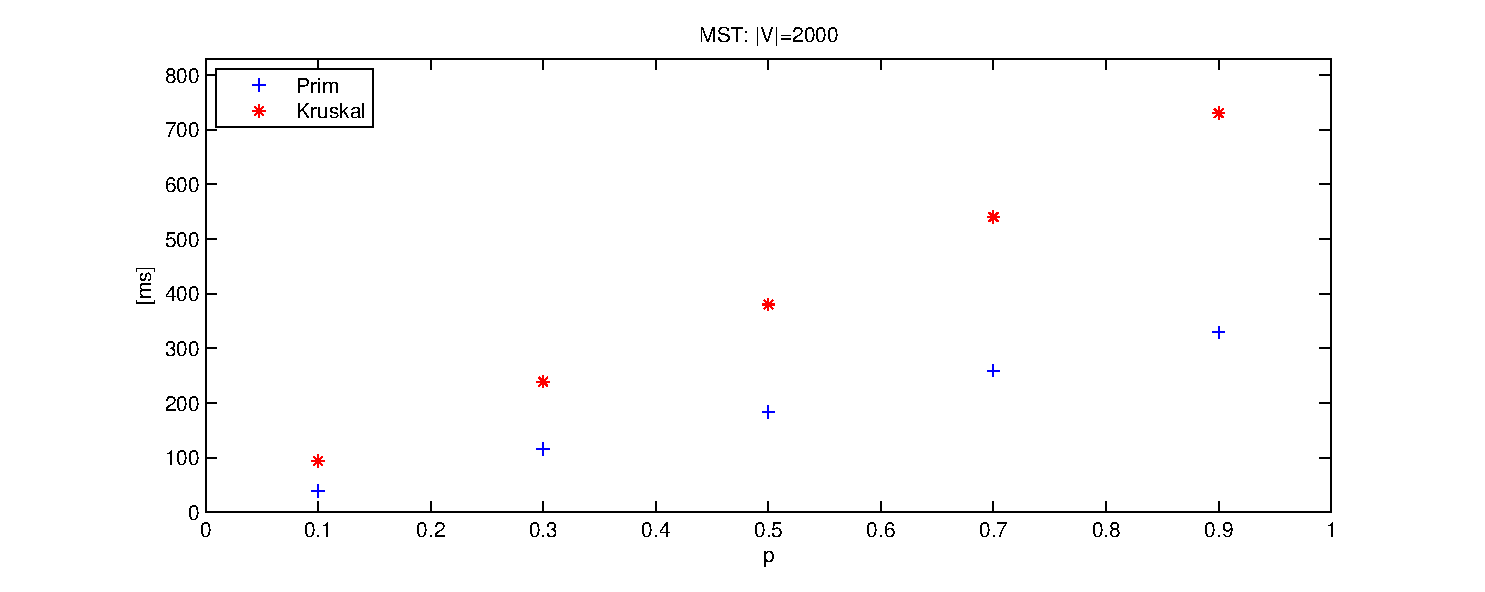
\includegraphics[width=165mm]{wykresy/v2000.eps}
\caption{\it{Czas wykonania algorytmów dla grafu zawierającego 2000 wierzchołków w zależności od prawdopodobieństwa wystąpienia krawędzi}}
\label{overflow}
\end{figure}

\begin{figure}[ht!]
\centering
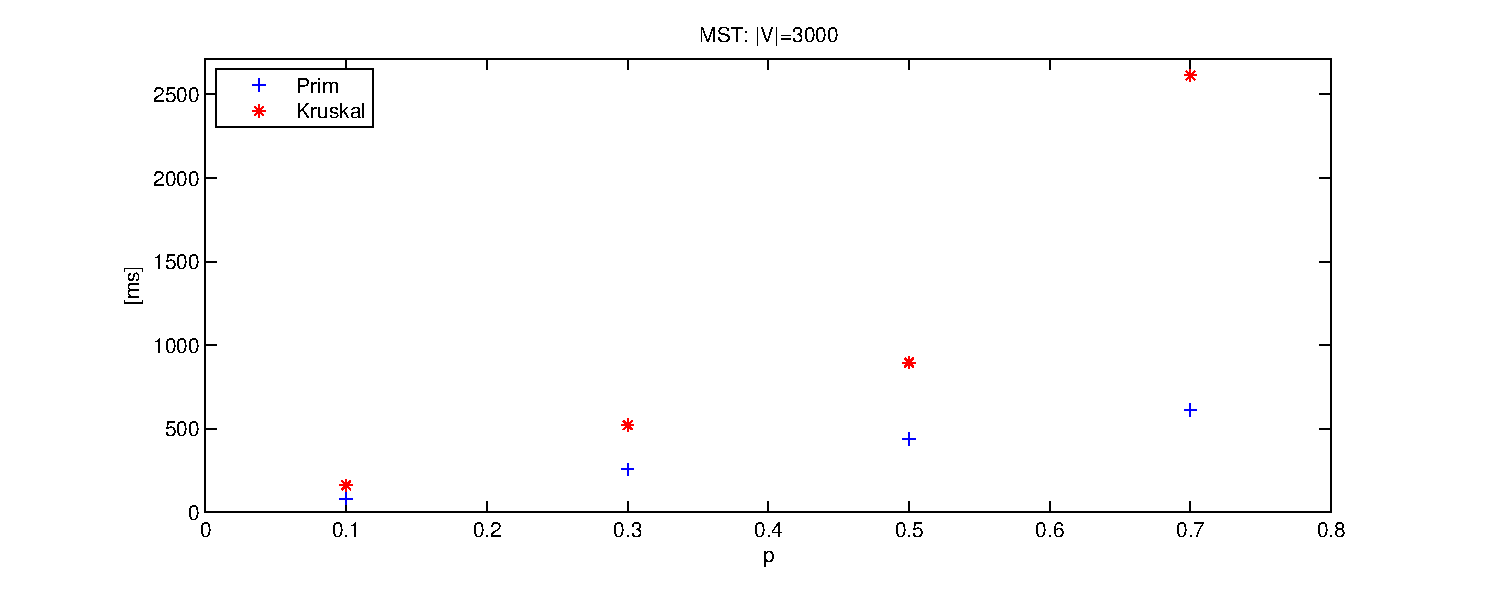
\includegraphics[width=165mm]{wykresy/v3000.eps}
\caption{\it{Czas wykonania algorytmów dla grafu zawierającego 3000 wierzchołków w zależności od prawdopodobieństwa wystąpienia krawędzi}}
\label{overflow}
\end{figure}


\subsection{Pamięć}

\begin{figure}[ht!]
\centering
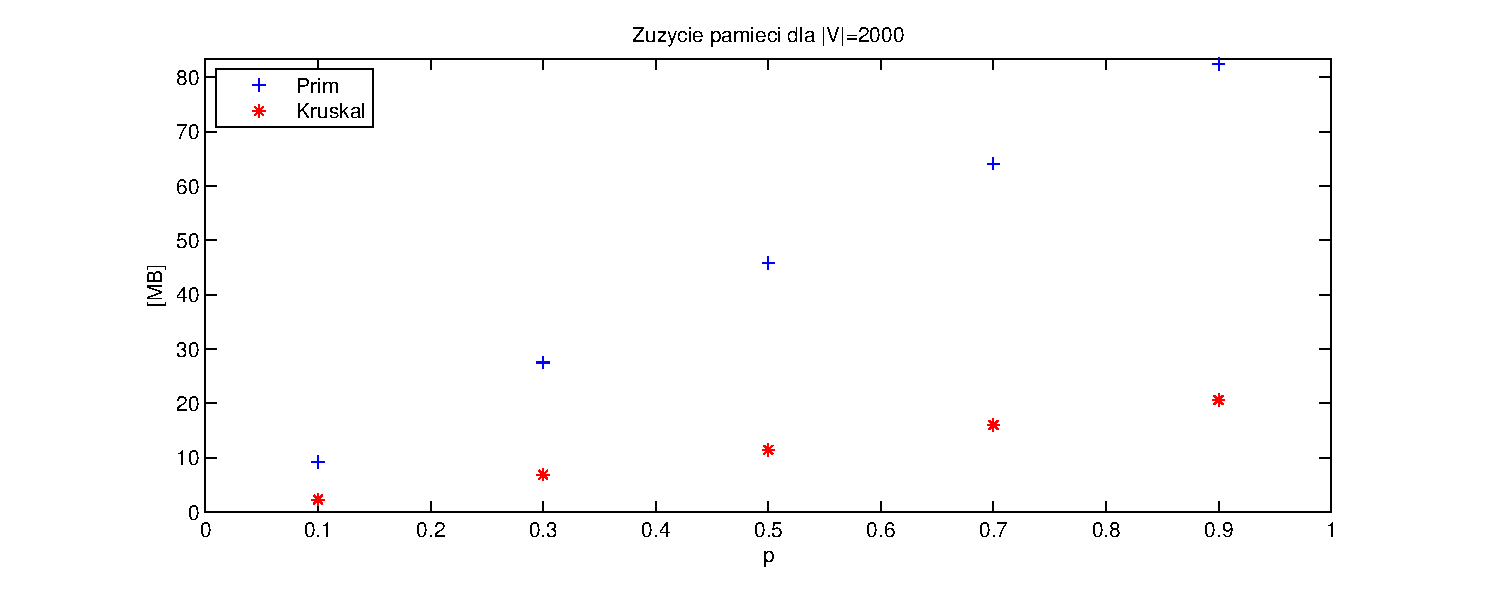
\includegraphics[width=165mm]{wykresy/mem.eps}
\caption{\it{Zużycie pamięci przez algorytmy dla grafu zawierającego 2000 wierzchołków w zależności od prawdopodobieństwa wystąpienia krawędzi}}
\label{overflow}
\end{figure}
\FloatBarrier
\section{Wnioski}






	





%BIBLIOGRAFIA
\nocite{*}
\renewcommand\refname{\section{Bibliografia}}
\bibliography{bibliografia}


\end{document}


